\documentclass[letterpaper,inpress,dvipsnames]{jdsart}

\setcounter{page}{1}
\pubmonth{July}
\pubyear{2022}
\volume{xx}
\issue{xx}
\doi{0000}


\usepackage[utf8]{inputenc}
\providecommand{\tightlist}{%
  \setlength{\itemsep}{0pt}\setlength{\parskip}{0pt}}


\usepackage{amsfonts,amsmath,amssymb,amsthm} 
\usepackage{booktabs} 
\usepackage{lipsum} 
\PassOptionsToPackage{dvipsnames}{xcolor} 
\newcommand{\svp}[1]{{\textcolor{ForestGreen}{#1}}} 
\newcommand{\tw}[1]{{\textcolor{Violet}{#1}}}

\begin{document}
\begin{frontmatter}

\title{Evaluating Perceptual Judgements on 3D Printed Bar Charts}
\runtitle{Perceptual Judgements on 3D Printed Bar Charts}

\author[1]{
  \inits{T.}
  \fnms{Tyler}
  \snm{Wiederich}  \thanksref{1}  \ead{twiederich2@huskers.unl.edu}}
\author[1]{
  \inits{S.}
  \fnms{Susan}
  \snm{VanderPlas}  \ead{susan.vanderplas@unl.edu}}

\thankstext[type=corresp,id=1]{Tyler Wiederich}
\address[1]{Department of Statistics, 
  \institution{University of Nebraska-Lincoln}, \cny{United States of America}}

\begin{abstract}
The use of 3D data visualizations has limitations when the third dimension does not convey any additional information to the viewer. Numerous studies advocate to avoid these types of graphs whenever possible, but these studies are almost entirely focused on the 2D projections of the 3D graphs. This paper describes the partial replication of a well-known paper in data visualization and its adaptation to focus on 3D printed bar charts. While current results from our study do not show differences between 2D and 3D graphs, we will use this study to provide students of a introductory statistics course hands-on experience with the research process.
\end{abstract}

\begin{keywords}
\kwd{graphics}\kwd{3D bar charts}\kwd{3D printing}.
\end{keywords}

\end{frontmatter}

\hypertarget{introduction}{%
\section{Introduction}\label{introduction}}

\hypertarget{elementary-graphical-tasks}{%
\subsection{Elementary Graphical Tasks}\label{elementary-graphical-tasks}}

\citet{cleveland_graphical_1984} published a paper that sets up the foundation for how accurately people extract quantitative information using elementary perceptual tasks (EPTs).
{\textcolor{ForestGreen}{Elementary Perceptual Tasks, according to these experiments,}} include {\textcolor{ForestGreen}{assessing}} graphical elements such as position along a common scale, length, angle, and volume{\textcolor{ForestGreen}{, and estimating the corresponding numerical value of these representations}}.
{\textcolor{ForestGreen}{XXX describe the overall results here XXX}}
{\textcolor{ForestGreen}{XXX Discuss that these results are primarily concerned with accuracy of numerical estimation, which is not always relevant. XXX}}
\citet{heerCrowdsourcingGraphicalPerception2010b} {\textcolor{ForestGreen}{replicated some parts of}} \citet{cleveland_graphical_1984} {\textcolor{ForestGreen}{in an online setting using Mechanical Turk, largely replicating the results of the original study while demonstrating the utility of the Mechanical Turk platform.}}

\textbf{OLD: Further studies have shown that 3D graphs are less accurate at portraying numeric information that 2D graphs \citep{barfield_effects_1989, fisher_data_1997}. In certain contexts and conditions, there is some research suggesting that 3D graphs may better encode information \citep{brath_3d_2014}.}

\hypertarget{d-graphical-perception}{%
\subsection{3D Graphical Perception}\label{d-graphical-perception}}

{\textcolor{ForestGreen}{Chart perception is often affected by the visual system's implicit assumption that visual stimuli are three-dimensional; after all, most of the visual input we process does come from a three-dimensional world, but charts are artificial and largely exist in two dimensions.}}

{\textcolor{ForestGreen}{This occasionally causes problems: the line-width illusion, for instance, has been attributed to implicit 3D perception of two-dimensional stimuli and can affect perception of error bands, candlestick plots, and Sankey diagrams}} \citep{vanderplasSignsSineIllusion2015, daySineIllusion1991, hofmannCommonAnglePlots2013}.

The use of 3D graphics have been explored in multiple studies.
\citet{fisher_data_1997} explored the preference of using either 2D or 3D graphs and found that subjects tended to use simpler 2D graphs when tasked with extracting information. \citet{barfield_effects_1989} compared 2D and 3D graphs presented on paper and on computers.
Their results showed that the accuracy of subject answers depended on their skill level.
Novice subjects were more accurate with 2D paper graphs and experienced managers were more accurate with 3D computer graphs.
For both experience levels, participants were more confident in their answers using 2D graphs over other presentations of data.
There are instances where 2D graphs perform better than 3D graphs, but there are times where 3D graphs may better encode information.
\citet{brath_3d_2014} highlights the intrinsic attributes of 3D graphs and its benefits when used appropriately with other 3D elements such as lighting and correct portrayal of data attributes.

{\textcolor{ForestGreen}{There is thus good reason to be wary of the use of three dimensions where only two are necessary to convey data. 
However, the situation is different now than it was in 1984 when Cleveland \& McGill published their seminal work; it has even changed since 2014. 
Digital graphics has developed quickly, along with the hardware necessary to support these software developments. 
As a result, we have much more natural rendering of 3D objects virtually, and we can also print graphics in three dimensions, moving the artificial charts into a more natural setting.
As a result, it is reasonable to reconsider the use of 3D charts, not only because of technological developments, but because these charts provide the opportunity to make visual graphics accessible to those with limited or absent vision.}}

Here, we provide the process of replication and modernization of testing perceptual judgments to 2D graphs, 3D graphs projected in 2D environments, and 3D printed bar graphs.

\hypertarget{selected-components-from-cleveland-and-mcgill}{%
\subsection{Selected Components from Cleveland and McGill}\label{selected-components-from-cleveland-and-mcgill}}

Cleveland and McGill provided a theory and tested for the ordering of perceptual importance for the elements of length, position, and angle.
Their first experiment, referenced as the position-length experiment, used five types of bar charts.
Two of these were grouped bar charts and the other three were stacked bar charts.
Each chart had two bars used for comparison and participants were asked to determine which bar was smaller and give their perceived ratio of the smaller bar to the larger bar.
The two grouped bar charts are for the perceptual element of position along a common scale, where one has zero distance between bars and the other has a fixed distance between bars.
These grouped bar charts will be referenced as adjacent and separated graph types in this paper, respectively.

Our study replicates the procedure for the comparisons of the two grouped bar charts, but with an objective of detecting differences in accuracy between 2D graphs, 3D digital graphs, and 3D printed graphs.

\hypertarget{methods}{%
\section{Methods}\label{methods}}

Our study is designed to replicate {\textcolor{ForestGreen}{and expand upon}} the position-length experiment from Cleveland and McGill as closely as possible.
In this section, we will discuss the replication process and the design of our modified version of this experiment.

\hypertarget{replicating-cleveland-and-mcgill}{%
\subsection{Replicating Cleveland and McGill}\label{replicating-cleveland-and-mcgill}}

The first step of replicating the position-length experiment was to determine the heights of the bars that participants use for comparisons.
These values for the bar heights are linear on a log scale and are given by

\[s_i=10\cdot 10^{(i-1)/12}, \qquad i=1,...,10\]

\textbf{OLD: The ratio of heights between the bars that were compared by Cleveland and McGill were 17.8, 26.1, 38.3, 46.4 (twice), 56.2, 68.1 (twice), and 82.5 (twice).}
\emph{NEW: Each graph presents two bars from the values given above where the participants are asked to judge the ratio of the smaller bar to the larger bar. The ratio of bars used by Cleveland and McGill were 17.8, 26.1, 38.3, 46.4 (twice), 56.2, 68.1 (twice), and 82.5 (twice).}
The exact numeric comparisons were not disclosed, but the comparison values used in our study were subjected to the constraints of having the same ratio values and that no value was used more than twice.

Each graph is presented so that there are ten bars where only two of the bars are marked for identification.
Cleveland and McGill did not specify the random process for the heights of the eight other bars, so we used a scaled Beta distribution with parameters that limit excessive noise around the bars used for comparisons. {\textcolor{ForestGreen}{XXX Indicate where code for this is available, as well as the data for each plot used in the study XXX}}
The aspect ratio of the plots is approximately 4:3.3, which was determined by measuring the pixels of a figure in Cleveland and McGill's paper.

\hypertarget{stimuli-construction}{%
\subsection{Stimuli Construction}\label{stimuli-construction}}

{\textcolor{ForestGreen}{XXX what limitations? What adjustments did we make? XXX}}

Due to limitations, creative adjustments were made from Cleveland and McGill's study to closely match both types of 3D charts (digital and 3D printed) to our 2D charts.
The graphs share a common layout {\textcolor{ForestGreen}{across all formats}}, where two groupings of five bars are identified by {\textcolor{ForestGreen}{"A" and "B", respectively, and circles and triangles are used to identify the bars participants should compare. Example graphs are shown in}}
Figure \ref{fig:plotTypes}.

\begin{figure}
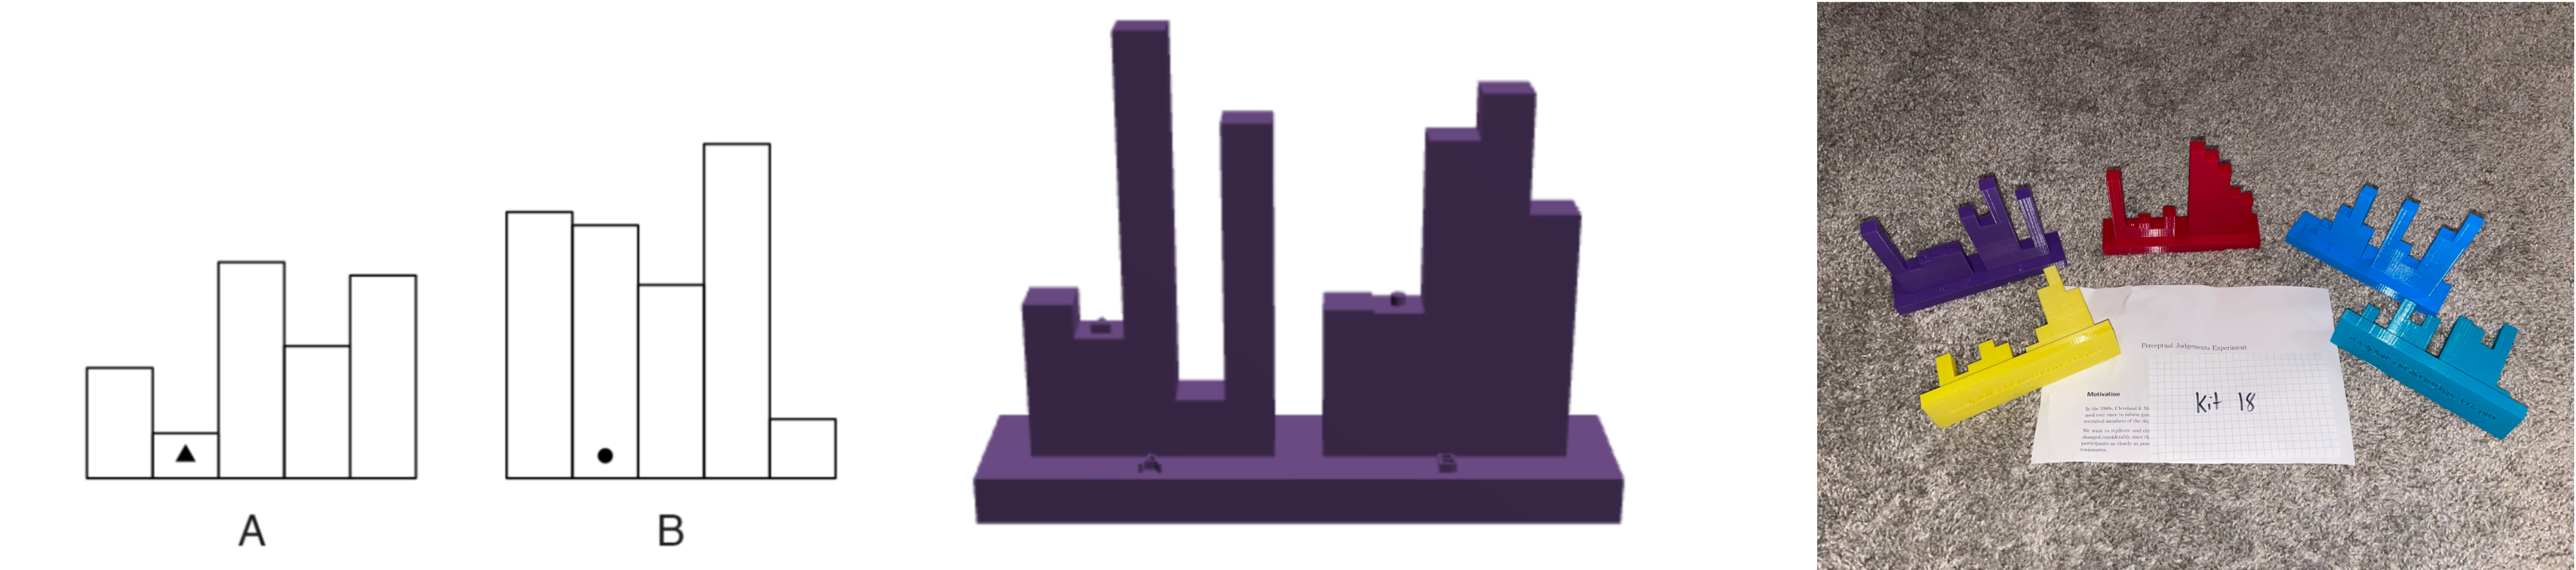
\includegraphics[width=1\linewidth]{plot-types} \caption{Two dimensional, two-dimensional digital rendering, and 3D-printed charts used in this study.}\label{fig:plotTypes}
\end{figure}

The ggplot2 \citep{ggplot2} package was utilized to create the 2D bar charts.
The scale axis was removed, leaving only the bars and a bar grouping identifier.
The bars used for comparisons had the identifying mark at a height of 5 out of 100 for the 2D plots, and the 3D plots had the identifying marks on top of the bars.

{\textcolor{ForestGreen}{The 3D renderings and 3D printed charts were both created using}} OpenSCAD \citep{kintelOpenSCADDocumentation2023}, {\textcolor{ForestGreen}{which creates STL files from markup describing the object's geometric composition. 
Charts were composed of a platform, raised labels for the A and B groups of bars, circle and triangle markers indicating the bars of interest, and the bars themselves; values for the bar heights were inserted into the markup using R}} \citep{R}.
{\textcolor{ForestGreen}{In addition, an ID code was engraved into the bottom of the platform to uniquely identify each object; this allows the researchers to ensure that the 3D printed charts are correctly allocated to stimulus sets.}}

{\textcolor{ForestGreen}{Digital renderings of the generated STL files were created using}} \citet{rgl} {\textcolor{ForestGreen}{, which integrates into}} \citet{shiny} {\textcolor{ForestGreen}{using the}} \citet{mozillafoundationWebGL2D3D2023} {\textcolor{ForestGreen}{extension}}.
{\textcolor{ForestGreen}{Rendered 3D charts were initially angled corresponding to the default 3D bar charts present in Microsoft Excel, but WebGL's interactivity allows the user to rotate, scale, and otherwise interact with the chart to change the angle. 3D renderings were colored to correspond to the 3D printed chart filament color.}}
{\textcolor{ForestGreen}{XXX discuss the lighting and rendering settings you used.}}

3D charts were printed with colored filament {\textcolor{ForestGreen}{corresponding to a specific}} ratio comparison{\textcolor{ForestGreen}{; this allowed researchers to visually assess kits to ensure that they contained five unique ratios}}.
{\textcolor{ForestGreen}{Colors corresponding to each ratio were assigned randomly to ensure that chart color provided no useful information about the ratio value.
As printed, the base of the chart was 13cm x 3cm x 1cm, with the highest bar rising 9.5cm above the chart base.
Raised letters and shapes were 2mm above the base or bar, respectively.}}

\hypertarget{experiment-design}{%
\subsection{Experiment Design}\label{experiment-design}}

Participants were provided a kit with five {\textcolor{ForestGreen}{3d-printed charts, comprising five}} of the seven unique ratio comparisons{\textcolor{ForestGreen}{; we then used the kit ID to ensure that participants saw computer-rendered charts with ratios corresponding to those in the kit of physical charts}}.
{\textcolor{ForestGreen}{This ensured that the experimental design was balanced across chart type and randomized with respect to the type of comparison (adjacent or separated).}}
{\textcolor{ForestGreen}{We printed graphs sufficient to create 21 kits of five 3d-printed charts each.}}

\begin{figure}
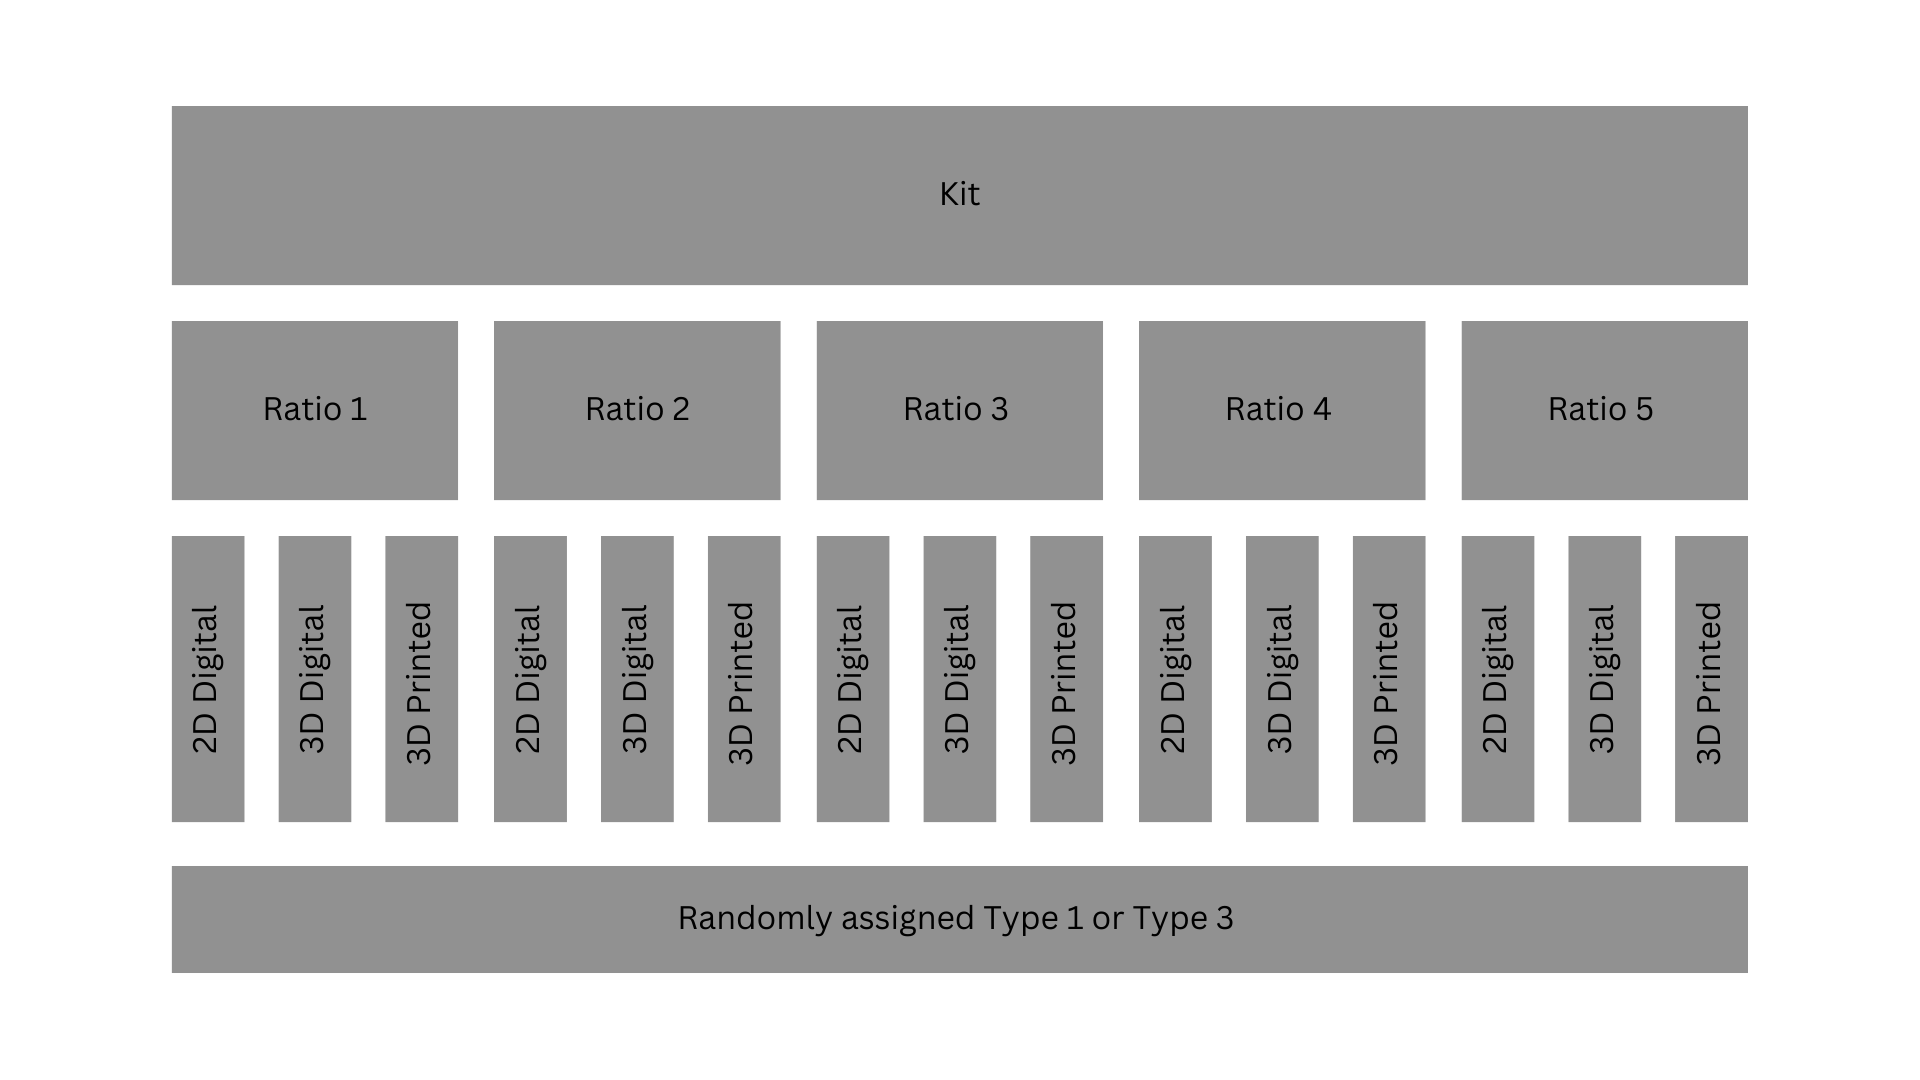
\includegraphics[width=6.4in]{study-design} \caption{A graphical representation of the study design. XXX is this accurate? Didn't we decide to do something like ensuring that either the smallest or largest ratio was included? You should show all 7 ratios, and indicate that we selected 5, as well. XXX}\label{fig:studyDesign}
\end{figure}

\hypertarget{participant-recruitment}{%
\subsection{Participant Recruitment}\label{participant-recruitment}}

{\textcolor{ForestGreen}{One interesting facet of}}

\citet{cleveland_graphical_1984}
{\textcolor{ForestGreen}{is the participant recruitment methodology: "For each experiment the subjects fell into two categories: (1) a group of females, mostly housewives, without substantial technical experience; (2) a mixture of males and females with substantial technical training and working in technical jobs. Most of the subjects in the position-length experiment participated in the positionangle experiment; in all cases repeat subjects judged the position-angle graphs first." It would seem likely that the authors recruited individuals within their respective departments as well as their wives.}}
In the spirit of replicating {\textcolor{ForestGreen}{the}} study, members of {\textcolor{ForestGreen}{the UNL}} Statistics department and their {\textcolor{ForestGreen}{spouses,partners, and roommates}} were asked to participate in our study{\textcolor{ForestGreen}{; this replicates the spirit of the original study without the implicit assumptions that graduate students and professors are (1) largely male, (2) are heterosexual, and (3) have unemployed partners}}.

\hypertarget{data-collection}{%
\subsection{Data Collection}\label{data-collection}}

{\textcolor{ForestGreen}{A Shiny applet was used for data collection, along with the provided kit of 3D printed charts.
Participants provided informed consent through the applet, and then were asked for demographic information (age, gender, education level). 
Then, participants were shown a "practice" page which allowed them to experiment with the data collection interface and practice estimating the ratio between the bars, as shown in}} Figure \ref{fig:practice}

\begin{figure}
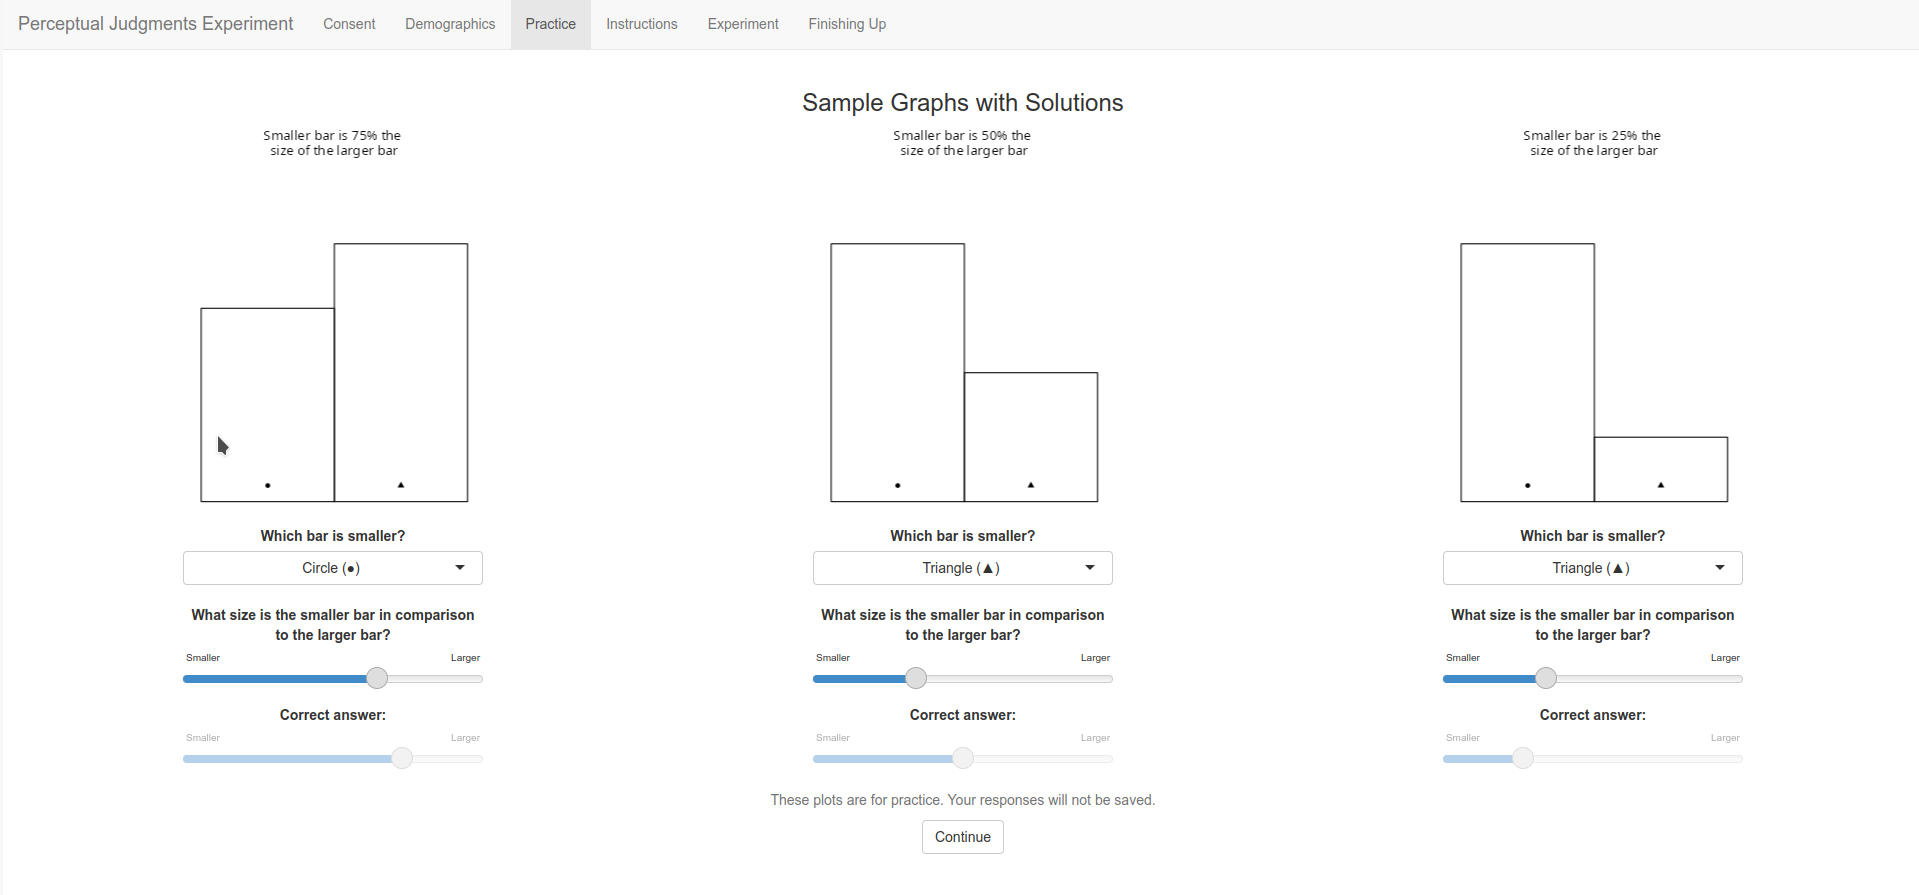
\includegraphics[width=6.4in]{03-Practice-2} \caption{Screenshot of Shiny application practice screen. Three 2D bar charts with different ratios were provided, along with sliders indicating the correct proportion. Participants could practice with the sliders and preview the questions that would be asked as part of the task.}\label{fig:practice}
\end{figure}

{\textcolor{ForestGreen}{Directly before the experiment started, participants were asked to provide the kit ID, along with directions indicating that if the instructions indicated that participants should use a 3D chart for a task, the participant should select a chart from the kit, enter the ID code of that chart from the bottom of the object, and complete the requested task.
Participants were also instructed to make quick judgments for each graph and not to measure or estimate ratios using physical objects.}}

\begin{figure}
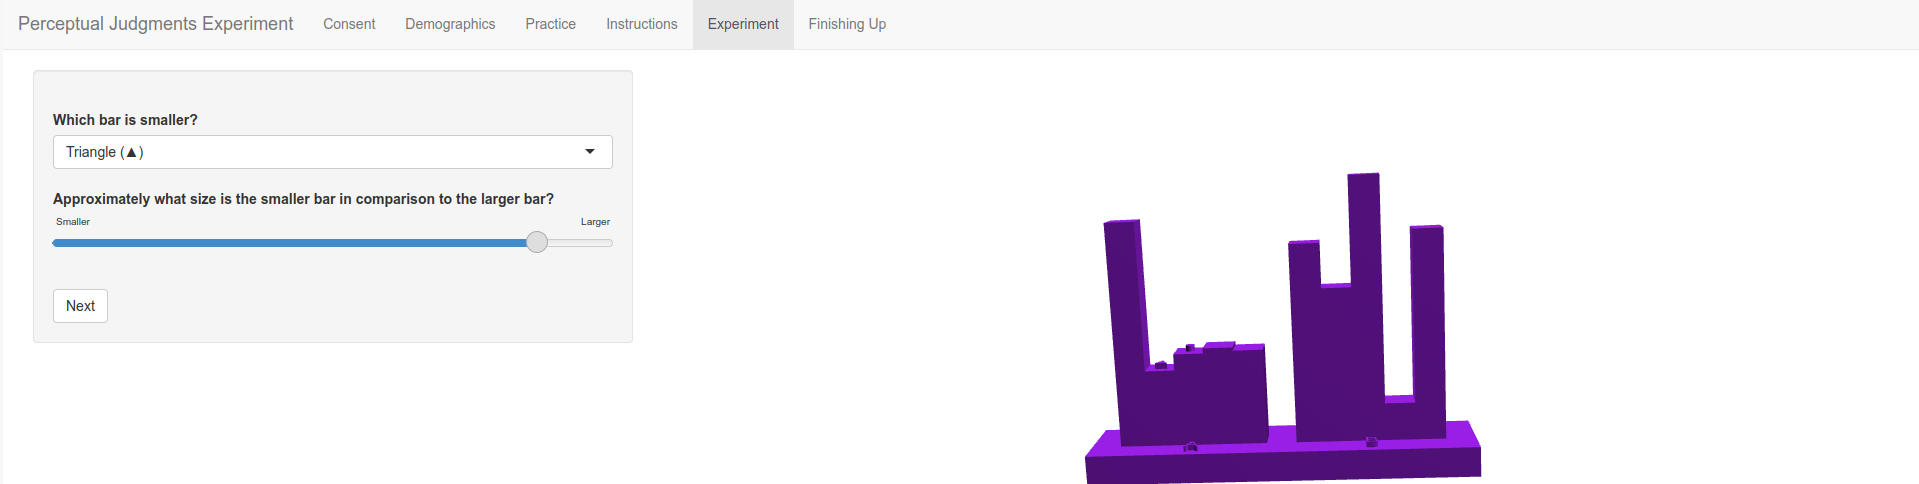
\includegraphics[width=6.4in]{05-Experiment-05-filled-in} \caption{Screenshot of the applet collecting data for a 3D rendered chart task. Participants were asked to select which bar (circle or triangle) was smaller, and then to estimate the ratio of the smaller bar to the larger bar.}\label{fig:experiment3dRender}
\end{figure}

{\textcolor{ForestGreen}{Each graph (or prompt, in the case of 3D printed charts) in the applet had two corresponding questions for participants to answer: first, participants were to identify the smaller bar by shape, and then, participants were to estimate the ratio of the size of the smaller bar to the size of the larger bar, as shown in}} Figure \ref{fig:experiment3dRender}.

\hypertarget{results}{%
\section{Results}\label{results}}

{\textcolor{ForestGreen}{XXX did C\&M use mixed effects models? If not, then you want to talk about the log2 part first, and then talk about why you used a mixed effects model. XXX}}

The data was analyzed with the same log error that was used by Cleveland and McGill. This is presented as the following linear mixed effects model.

\[y_{ijklm}=\mu+S_i+R_j+G(R)_{(k)j}+T_l+\epsilon_{ijklm}\]

\noindent where

\begin{itemize}
\item
  \(y_{ijklm}=\log_2(|\text{Judged Percent} - \text{True Percent}|+1/8)\)
\item
  \(S_i\sim N(0,\sigma^2_S)\) is the effect of the \(i^{th}\) subject
\item
  \(R_j\) is the effect of the \(j^{th}\) ratio
\item
  \(G(R)_{(k)j}\) is the effect of the \(k^{th}\) graph type nested in the \(j^{th}\) ratio
\item
  \(T_l\) is the effect of the \(l^{th}\) comparison type
\item
  \(\epsilon_{ijklm}\sim N(0,\sigma^2_\epsilon)\) is the random error
\end{itemize}

A total of 39 subjects participated in the study. {\textcolor{ForestGreen}{XXX Need to add in demographics - how many of each group? Breakdown by sex, age? XXX}}
All responses that incorrectly identified the smaller bar were removed.
No differences were detected for the true ratio of bars (p-value = .689), whether the bars were adjacent or separated (p-value = .220), or for the plot nested within the true ratio (p-value = .837).

\hypertarget{discussion-and-future-work}{%
\section{Discussion and Future Work}\label{discussion-and-future-work}}

Previous work in 3D graphics would suggest that the errors for the 3D graphs would be larger than the errors for the 2D graphs. {\textcolor{ForestGreen}{While we did not find any significant results indicating that 3D graphs are read less accurately, there are two possibilities that might account for this discrepancy. The first is that this study is underpowered - the effect size is small, and our 39 participants were insufficient; the original study included 51 participants, which is slightly larger. The second possibility is more interesting: we examined 3D charts using rendered 3D graphs and 3D printed charts; both of these options allow for participants to interact with the chart, rotating it, and generally perceiving it as one might perceive any other 3D, real, object. This is a far cry from the 3D perspective charts in the original study, which have a fixed angle and perspective and are thus not equivalent to our 3D charts. Future studies should include an additional fixed 3D perspective bar chart, which will at least enable us to examine whether modern 3D rendering environments allow for more accurate conclusions than fixed 3D perspectives.}}

Future iterations of this study will include ``traditional'' 3D graphs created by Microsoft Excel and provide the option for online participants to remove the 3D printed graphs from the graphs in their kit. {\textcolor{ForestGreen}{Stimuli, code, and data for this experiment are provided at ... new repository set up to correspond to this paper ... along with instructions for replicating the analysis.}}

\bibliography{JDS2023.bib}
\bibliographystyle{jds}


\end{document}
